%%%%%%%%%%%%%%%%%%%%%%%%%%%%%%%%%%%%%%%%%%%%%%
%                insertmeeting
% 1) Title (something creative & funny?)
% 2) Date (MM/DD/YYYY)
% 3) Location (ex. Hagerty High School)
% 4) People/Committees Present 
% 5) Picture 
% 6) Start Time & Stop Time (ex. 12:30AM to 4:30PM)
%%%%%%%%%%%%%%%%%%%%%%%%%%%%%%%%%%%%%%%%%%%%%%
\insertmeeting 
	{Picking Up the Pace} 
	{11/22/21}
	{Hagerty High School}
	{Clayton, Nathan, Ritam}
	{Images/RobotPics/robot.jpg}
	{10:30 - 12:45}
	
\hhscommittee{General}
\noindent\hfil\rule{\textwidth}{.4pt}\hfil
\subsubsection*{Goals}
\begin{itemize}
    \item finish designing intake
    \item Find correct belt for intake
    \item Start printing parts

\end{itemize} 

\noindent\hfil\rule{\textwidth}{.4pt}\hfil

\subsubsection*{Accomplishments}
it's finally Thanksgiving break, which, aside from turkey, means no school! Although this means that we will have no mandatory meetings, those of us who aren't going on vacation are still hoping to get lots of progress made. The progress made today will be on the intake’s CAD which was started at the last meeting, but is still incomplete. 
Most of what needs to be completed is the coaxial arm and belt mechanism. We started by creating the main structure of the roller arm, which we plan to 3d print. To improve its structural integrity, we added ribs going across the bottom of  the roller arm. In addition to this, we added pocketing holes and some supports for a color sensor that will allow our software team to know if there is a block in the intake autonomously(Figure \ref{fig:pic1}). 
With the arm completed, we created a simple roller with a hex bore that we will 3d print and wrap in surgical tubing (Figure \ref{fig:pic2}). Because this roller is .75 inches in diameter, our pulley must have a diameter around or below .75 inches to keep it from getting in the way when we intake a block. We started out assuming we would use an XL belt as we have been on most of the other parts of the robot, but we found that the minimum pulley size for it to be reliable is about 1 inch in diameter, which is just a little bit too big. Finding this, we set out to find alternative belts that can work with pulleys of smaller diameters. We came across options like v-belt pulleys, but they are hard to find at a scale that works with our intake design. After looking for a while, our mentor gave us the idea of using o-ring belts, which are round rubber tubes that can be used as belts if tensioned correctly. Looking online, we found that GoBilda had pulleys that could be bought  that work with o-ring belts. Instead of buying these and waiting for them to ship, we decided to recreate them in cad and 3d print them. This way we could also add a hex bore that would allow us to easily attach it to a hex shaft (Figure \ref{fig:pic3}). After that, we designs some laser cut parts that would block the arm from pivoting too far down. We also attached a hole where we can attach a rubber band to help tension the arm downwards. The only part that left us to create was the bottom fiberglass plate. Because we will cut this by hand it isn’t essential that we create it in CAD, but we decided to add it anyway (Figure \ref{fig:pic4}).
Now that all the parts were created, we added them all into the assembly to ensure they fit together correctly(Figure \ref{fig:pic5}). Finding no errors, we are calling the intake CAD complete for now!
 

\begin{figure}[ht]
\centering
\begin{minipage}[b]{.48\textwidth}
  \centering
  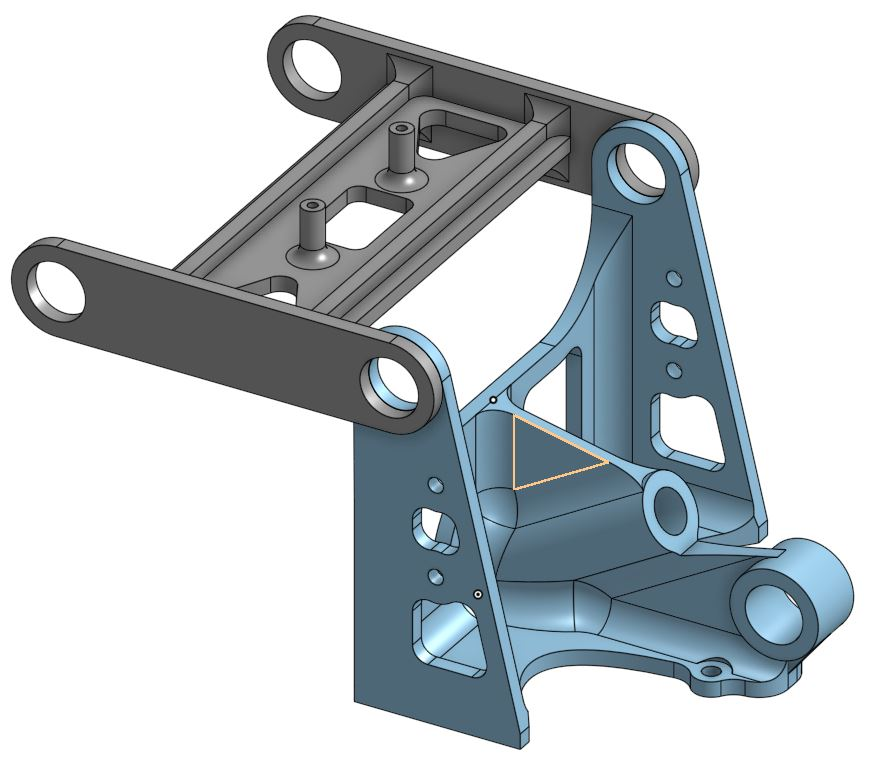
\includegraphics[width=0.95\textwidth]{Meetings/November/11-22-21/11-22-21_CAD_Figure1 - Nathan Forrer.JPG}
  \caption{Added mounting areas for a color sensor}
  \label{fig:pic1}
\end{minipage}%
\hfill%
\begin{minipage}[b]{.48\textwidth}
  \centering
  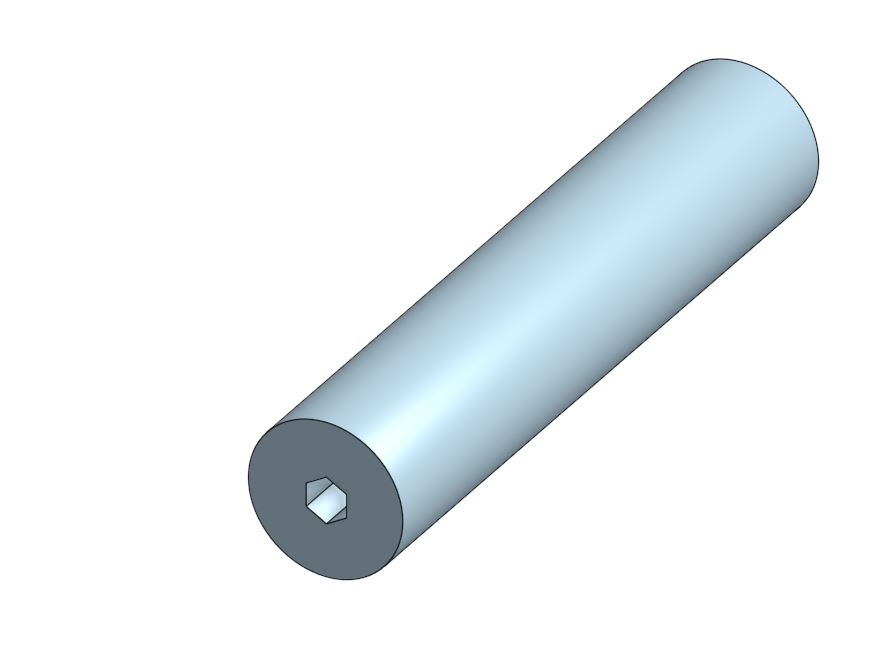
\includegraphics[width=0.95\textwidth]{Meetings/November/11-22-21/11-22-21_CAD_Figure2 - Nathan Forrer.JPG}
  \caption{Roller to wrap in surgical tubing}
  \label{fig:pic2}
\end{minipage}
\end{figure}

\begin{figure}[ht]
\centering
\begin{minipage}[b]{.48\textwidth}
  \centering
  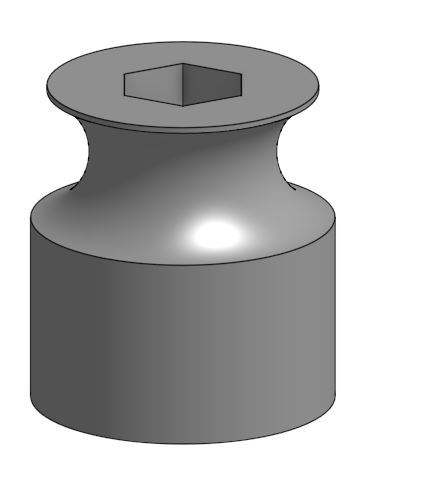
\includegraphics[width=0.95\textwidth]{Meetings/November/11-22-21/11-22-21_CAD_Figure3 - Nathan Forrer.JPG}
  \caption{Our custom hex hub}
  \label{fig:pic3}
\end{minipage}%
\hfill%
\begin{minipage}[b]{.48\textwidth}
  \centering
  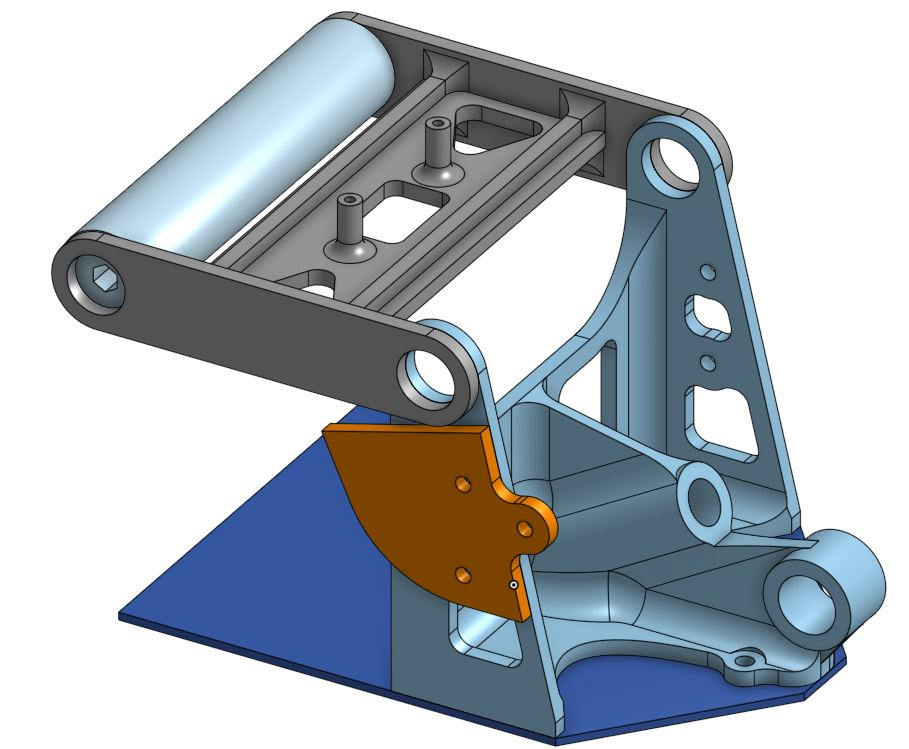
\includegraphics[width=0.95\textwidth]{Meetings/November/11-22-21/11-22-21_CAD_Figure4 - Nathan Forrer.JPG}
  \caption{The new fiberglass plate}
  \label{fig:pic4}
\end{minipage}
\end{figure}


\begin{figure}[htp]
\centering
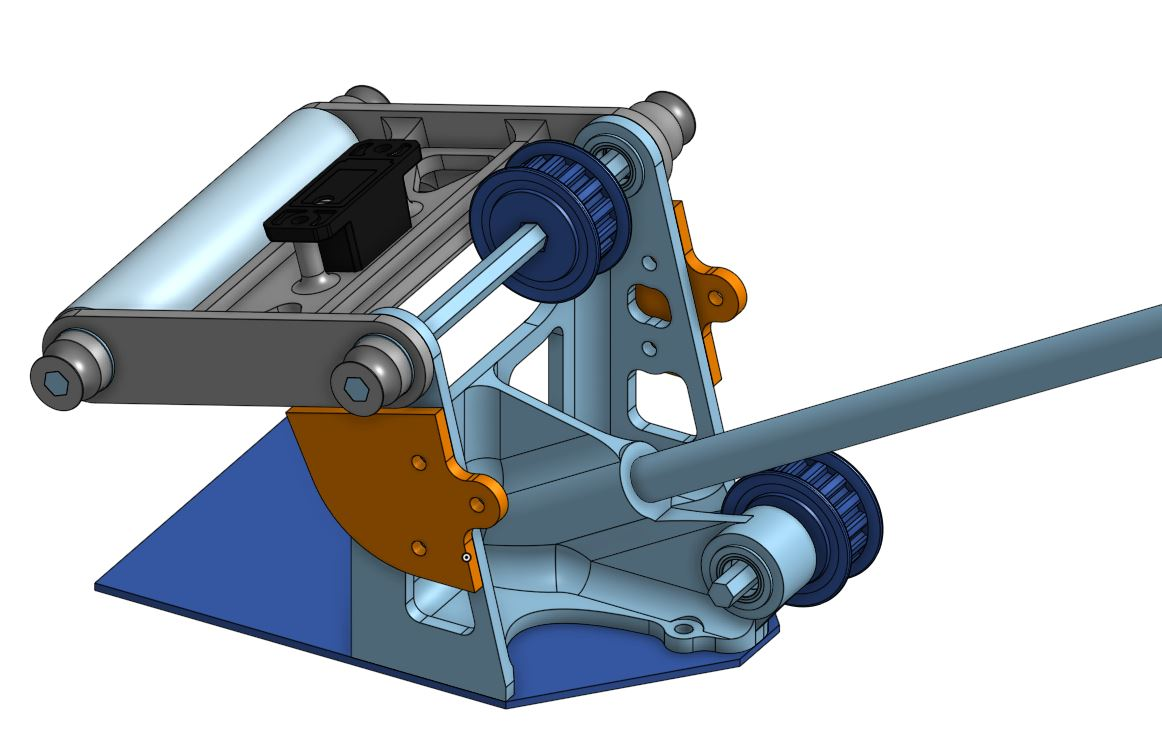
\includegraphics[width=0.95\textwidth, angle=0]{Meetings/November/11-22-21/11-22-21_CAD_Figure5 - Nathan Forrer.JPG}
\caption{The finished assembly}
\label{fig:pic5}
\end{figure}


\whatsnext{
\begin{itemize}
    \item Start printing parts
    \item Find correct o-ring belt size
\end{itemize} 
}

